\documentclass[xcolor=dvipsnames]{beamer}

\usepackage{etex}

\include{header}
\definecolor{darkgreen}{rgb}{0,0.5,0}
\definecolor{black    }{rgb}{1,1,1}
\definecolor{darkyellow}{rgb}{.8,.6,.04}
\newcommand{\red}  [1]{\textcolor{red}      {#1}}
\newcommand{\blue} [1]{\textcolor{blue}     {#1}}
\newcommand{\green}[1]{\textcolor{darkgreen}{#1}}
\newcommand{\RED}  [1]{\textcolor{red}      {#1}}
\newcommand{\BLUE} [1]{\textcolor{blue}     {#1}}
\newcommand{\GREEN}[1]{\textcolor{darkgreen}{#1}}
\newcommand{\white}[1]{\textcolor{white}    {#1}}
\newcommand{\black}[1]{\textcolor{black}    {#1}}
\newcommand{\dyell}[1]{\textcolor{darkyellow}{#1}}
\newcommand{\cyan}[1]{\textcolor{cyan}{#1}}
\newcommand{\PURPLE}{\textcolor{magenta3}}
\newcommand{\br}[1]{{\bf\red{#1}}}
\newcommand{\bb}[1]{{\bf\blue{#1}}}
\newcommand{\bg}[1]{{\bf\green{#1}}}
\newcommand{\yb}[1]{\colorbox{yellow}{#1}}

\newcommand{\var}[1]{\ensuremath{\boldsymbol{#1}}}
\newcommand{\obj}[3]{
  & \mbox{#1}      &            % the model name
  #2 \phantom{M}   & #3 &       % second column for the objective function
  &  &                          % third column is empty
}
\newcommand{\con}[3]{           % simple constraint
  & &                           % first column is empty
  #1 \phantom{M}   & #2 &       % second column for the constraints
  \phantom{M} #3   &  &         % third column for the domain
} 

\newcommand{\conu}[2]{          % allow the user to align the second column
  & &                           % first column is empty
  #1 &                          % second column for the constraints
  \phantom{M} #2  &  &          % third column for the domain
} 


\usepackage{tikz,pgfplots,pgfplotstable}
%\usepackage{epsf,amsmath,amssymb,amsfonts}
\usepackage{movie15}
\usepackage{graphicx}
\usepackage{epsfig}
\usepackage{float}
\usepackage{caption}
\usepackage{subcaption}
\usepackage{hyperref}
\usepackage{comment}
\usepackage{color, colortbl}
\definecolor{LRed}{rgb}{1,.8,.8}
\usepackage{rotate}
\usepackage{BeamerColor}
\usepackage{paralist}
\usepackage{algorithmicx,algpseudocode}
%---------------------------------------------------------------------------
%Tomo USER DEFINED MACROS

%Response to review macros
\newcommand{\bfc}[1]{{\bf \underline{Response:} }\textnormal{#1}}
\usepackage{color}
% \definecolor{gray}{rgb}{0.5,0.5,0.5}

%%% The following commands are for a marked up version 2, comment for markedup
 % \newcommand{\addone}[1]{\textcolor{violet}{#1}}
 %  \newcommand{\changeone}[1]{\textcolor{red}{#1}}
 %  \newcommand{\doneone}[2][]{\todo[#1]{#2}}
%%% unmarkedup
  \newcommand{\addone}[1]{#1}
  \newcommand{\changeone}[1]{#1}
  \newcommand{\doneone}[2][]{}
%%% The following commands are for an unmarked up version 1, comment for markedup
\newcommand{\added}[1]{#1}
\newcommand{\changed}[1]{#1}
\newcommand{\removed}[1]{}
\newcommand{\done}[2][]{}
\newcommand{\mdone}[1]{}


%Paper body notation
\newcommand{\R}{\mathbb{R}} % reals
\newcommand{\cE}{{\mathcal{E}}} % This will be the set of elements
\newcommand{\cV}{{\mathcal{V}}} % This will be the set of voxels
\newcommand{\cN}{{\mathcal{N}}} % This will be the non-binding set
\newcommand{\cI}{{\mathcal{I}}} % This will be the set of energy channels
\newcommand{\mcT}{{\mathcal{T}}} % This will be the set of energy channels
\newcommand{\cU}{{\mathcal{U}}} % This will be the set of upstream voxels
\newcommand{\cA}{\mathcal{A}} % Active set
\newcommand{\I}[1]{\mathbb{I}_{#1}} % The indicator function
\newcommand{\ones}{\mathbf{1}} % Vector ones
\newcommand{\At}{  A^{E,\theta,\tau}} % Attenuation array
\newcommand{\A}{ {\bf A}} % Attenuation array
\newcommand{\bd}{ {\bf d}} 
\newcommand{\bx}{ {\bf x}} 
\newcommand{\Fl}{\pmb{\mathbf{\rho}}} % Fluorescence emitted array
\newcommand{\Le}{{\bf L}} % length array
\newcommand{\m}{{\bf m}} % M
\newcommand{\cW}{{\mathcal{W}}}
\newcommand{\bcW}{\pmb{\mathbf{\cW}}}
\newcommand{\X}{{\bf X}}
\newcommand{\bc}{{\bf c}}
\newcommand{\byi}{{\bf y_i}}
\newcommand{\bmi}{{\bf m_i}}
\newcommand{\Y}{{\bf Y}}
\newcommand{\ds}{{\displaystyle}}
\newcommand{\argmin}{\operatornamewithlimits{argmin}}
\newcommand{\MD}[1]{{\bf D}_{\theta,\tau}^\mathit{#1}}  % experimental
\newcommand{\MDRi}{D_{\theta,\tau,\iota}^\mathit{R}}  % experimental
\newcommand{\D}[1]{{\bf D}^\mathit{#1}}  % experimental
% data XRF
\newcommand{\MDT}{D_{\theta,\tau}^\mathit{T}}  % experimental data XRF
\newcommand{\tMD}[1]{\pmb{\mathbf{\tilde{D}}}_{\theta,\tau}^\mathit{#1}}  %
% experimental data

\newcommand{\FM}[1]{{\bf F}_{\theta,\tau}^\mathit{#1}} % forward model
\newcommand{\FMRi}{F_{\theta,\tau,\iota}^\mathit{R}} % forward model
% for XRF
\newcommand{\FMT}[1]{{#1}_{\theta,\tau}^\mathit{T}}% forward model for XRT
\newcommand{\J}[1]{{\bf J}^\mathit{#1}} % forward model for XRF


%% macros from CVT
\def \ds          {\displaystyle}
\def \rmd         {{\rm d}}
\def \be          {{\bf e}}
\def \bF          {{\bf F}}
\def \bI          {{\bf I}}
\def \bn          {{\bf n}}
\def \bff         {{\bf f}}
\def \bdf         {{\bf df}}
\def \bdT         {{\bf dT}}
\def \bT          {{\bf T}}
\def \cT          {{\cal T}}
\def \bU          {{\bf U}}
\def \bu          {{\bf u}}
\def \bv          {{\bf v}}
\def \bV          {{\bf V}}
\def \bX          {{\bf X}}
\def \by          {{\bf y}}
\def \bY          {{\bf Y}}
\def \bz          {{\bf z}}
\def \bZ          {{\bf Z}}
\def \bW          {{\bf W}}
\def \bZt         {{\bf \widetilde Z}}
\def \bzi         {{\bz}_i}
\def \bzs         {{\bz}^*}
\def \bzis        {{\bz}_i^*}
\def \bzin        {\{\bzi\}_{i=1}^k}
\def \cf          {{\cal F}}
\def \cg          {{\cal G}}
\def \ch          {{\cal H}}
\def \vi          {{V_i}}
\def \vin         {\{\vi\}_{i=1}^k}
\def \Babs        {{\Big|}}
\def \Bl          {{\Big(}}
\def \Br          {{\Big)}}
\def \Bleft       {{\Big[}}
\def \Bright      {{\Big]}}
\def \p           {\partial}
\def \N           {{\mathbb N}}
\def\y            {{\bf y}}
\def \tN          {{\widetilde{N}}}
\def \tD          {{\widetilde{D}}}

\def \proofnote #1{\footnote{{\bf Note: #1}}}
\def \norm      #1{\left\|\,#1\,\right\|}
\def \set       #1{\left\{\,#1\,\right\}}
\def \tr          {^T}
\def \IhH         {I_h^H}
\def \IhHb        {{\hat I}_h^H}
\def \IHh         {I_H^h}
\def \vbar        {\bar v}
\def \zhbar       {\bar z_h}
\def \zHbar       {\bar z_H}
\def \zhplus      {z_h^+}
\def \zHplus      {z_H^+}

\newcommand{\C}{{\bf C}}
\newcommand{\bmu}{\mathbf{\pmb{\mu}}} % This is for voxel attenuation
\newcommand{\lmu}{\tilde{\mu}}
\newcommand{\cbmu}{{\textcolor{red}{\bmu^E}}}
\newcommand{\blambda}{\pmb{\mathbf{\lambda}}}
\renewcommand{\theequation}{\thesection.\arabic{equation}}

\newtheorem{alg}{Algorithm}[section]
\newtheorem{thm}{Theorem}[section]
\newtheorem{lem}[thm]{Lemma}
\newtheorem{cor}[thm]{Corollary}
\newtheorem{pro}{Proposition}[section]
\newtheorem{defn}{Definition}[section]
\newtheorem{asp}{Assumption}[section]
\newtheorem{rmk}{Remark}[section]
\newtheorem{exmp}{Example}[section]

\newcommand{\SNote}[1]           % For Stefan's margin notes
{\textcolor{blue}{#1}\marginpar{\textcolor{blue}{SW $\longleftarrow$}}}
\newcommand{\cF}{\mathcal{F}}

\graphicspath{{./images/}}
\usebackgroundtemplate{\includegraphics[width=\paperwidth]{NormalANLBlue}}

\setbeamercolor{block title}{bg=LightSteelBlue,fg=blue}  % bg=background, fg= foreground
\setbeamercolor{block body}{bg=azure1,fg=black}          % bg=background, fg= foreground
\setbeamercolor{alerted text}{fg=white,bg=red}
\newcommand{\boxalert}[1]{{%
  \usebeamercolor{alerted text}\colorbox{bg}{\alert{#1}}%
}}
%%%%%%%%%%%%%%%%%%%%%%%%%%%%%%%%%%%%%%%%%%%%%%%%%%%%%%%%%%%%%%%%%%%%%%%%
\hypersetup{%
  pdftitle={Optimization Approach for Tomographic Inversion from Multiple Data Modalities},%
  colorlinks=true,
  linkcolor=Blue,
  urlcolor=Red }

% -- TITLE PAGE --
\title{Accelerating Halo Center Finding }
\author{Zichao (Wendy) Di, Salman Habib, Steve Rangel, and Stefan Wild}
%\subtitle[AMS]{GMU Applied Math Seminar}
\institute[Argonne]{Mathematics \& Computer Science Division\\ Argonne National Laboratory}
\date{}
%%%%%%%%%%%%%%%%%%%%%%%%%%%%%%%%%%%%%%%%%%%%%%%%%%%%%%%%%%%%%%%%%%%%%%%%

\begin{document}

%%%%%%%%%%%%%%%%%%%%%%%%%%%%%%%%%%%%%%%%%%%%%%%%%%%%%%%%%%%%%%%%%%%%%%%%
% ... Title Page
\setbeamertemplate{footline}{}
{
  \usebackgroundtemplate{\includegraphics[width=\paperwidth]{TitleANLBlue}}
  \frame{\titlepage}
}
%%%%%%%%%%%%%%%%%%%%%%%%%%%%%%%%%%%%%%%%%%%%%%%%%%%%%%%%%%%%%%%%%%%%%%%%

\setbeamertemplate{footline}[frame number]{}

% ========================================
% FRAME: overview
% ========================================
 \begin{frame}
   \frametitle{Outline}
   \tableofcontents
 \end{frame}

% ========================================
% main slides come here
% ========================================

%%%%%%%%%%%%%%%%%%%%%%%%%%%%%%%%%%%%%%%%%%%%%%%%%%%%%%%%%%%%%%%%%%%%%%%%%%%%%%
\section{Introduction of Halo}
%  \begin{frame}
%    \frametitle{Outline}
%    % \tableofcontents[currentsection]
%  \end{frame}

\frame{
\frametitle{Halo Analysis}
\begin{itemize}
  \item An important and time-consuming analysis in halo analysis is to find halos and the centers of those halos.
  \item The friend-of-friends (FOF) halo: particles are ``linked`` together if their distance is smaller than a given threshold, called ''linking length``. 
  \item FOF halos do not intersect, meaning that a particle can be assigned uniquely to just one FOF halo. 
  \item substructure defined by smaller linking length lies completely in the host halo. 
\end{itemize}
}

\frame{
\frametitle{Illustration}
\begin{columns}
\column{2.5in}
\begin{figure}[H]
\includegraphics[scale=0.45]{FOFgroups-bridge-nointersect.png}
\caption{FOF halos can not intersect, if two halos are close enough, they are combined as one}
\end{figure}
\column{2.5in}
\begin{figure}[H]
\centering
    \includegraphics[scale=0.45]{FOFgroups-sub-linklength.png}
     \caption{FOF halos with different linking lengths (yellow, orange, violet)}
\end{figure}
\end{columns}
}

\frame{
\frametitle{Halo Centers}
\begin{itemize}
\item Most connected particle (MCP) center: the aprticle within a halo with the most ``friends''.
\item Most bound particle (MBP) center: the particle within a halo with the lowest potential, where the potential for a given particle is computed as the sum over all other particles of the negative of mass divided by distance.
 $$ MBP=\min_i \ds\sum_{j\neq i}\frac{-m_j}{d(X_i,X_j)}$$
 where $X_i$ is the $i$-th particle, $m_i$ is its corresponding mass, and $d(X_i,X_j)$ is the Euclidean distance between particles $X_i$ and $X_j$. 
\end{itemize}
}

\frame{
\frametitle{Illustration}
\begin{figure}[H]
\centering
    \includegraphics[scale=0.7]{MBP_MCP.png}
    \caption{Illustration of MBP and MCP on halos}
\end{figure}
}

\section{Finding MBP}
\frame{
\frametitle{Existing Approaches}
\begin{itemize}
\item Common practice: brute force which ends in $O(N_p^2)$ complexity where $N_p$ is the total number of particles in a targeted halo.
\item Our goal: accelerate the process of MBP finding by recursive method.
\end{itemize}
\begin{figure}[H]
\includegraphics[scale=0.5]{naive.eps}
\end{figure}
}

\frame{
\frametitle{Proposed Recursive Method}
{\footnotesize
\begin{algorithmic}[]
\Procedure {$MBP=recursive\_localMBP(X,m)$}{}
\State{tree=kdtree(X).}
\State {\bf If $(level=1)$}
\State Select uniformaly distributed random indices $\tilde{i}$ from $[1,\dots,N_p]$ as $Seeds$.
\State For each $\tilde{i}$, $IDX=rangesearch(tree,X_{\tilde{i}},\varepsilon)$, where $\varepsilon$ is the neiborhood radius provided for tree search, and $IDX$ is the index function to indicate which particles are friends of $X_{\tilde{i}}$. Calculate $\tilde{BP}_{\tilde{i}}=\ds\sum_{\{j|IDX\neq j\}}\frac{-m_j}{d(X_{\tilde{i}},X_j)}$, where $\tilde{BP}$ denotes local bounded potential. 
\State Update $Seeds$ as local peaks of the $\tilde{BP}$ map, and find $\tilde{MBP}$ as the minimum of $\tilde{BP}$ map. 

\State {\bf Else}

\State for each $\tilde{i}$ in $Seeds$, calculate $IDX_{\tilde{i}}=rangesearch(tree,X_{\tilde{i}},\tilde{\varepsilon})$.

\State Calculate $\tilde{BP}$ for each particle in $IDX_{\tilde{i}}$ for each $\tilde{i}$.
\State Set $\tilde{MBP}_0=\tilde{MBP}$.
\State Find $\tilde{MBP}$ as the minimum of $\tilde{BP}$ map. 
\State if $\tilde{MBP}_0=\tilde{MBP}$, stop the procedure; else, $level=level+1$.
\EndProcedure
\end{algorithmic} 
}
}

\section{Numerical Results}
\frame{
\frametitle{Algorithm Illustration on 2D halo}
\begin{columns}
\column{1.2in}
\begin{figure}[H]
\includegraphics[scale=0.43]{2d_1}
\end{figure}
\column{1.2in}
\begin{figure}[H]
\centering
    \includegraphics[scale=0.43]{2d_2}
\end{figure}
\column{2.2in}
\begin{figure}[H]
\centering
    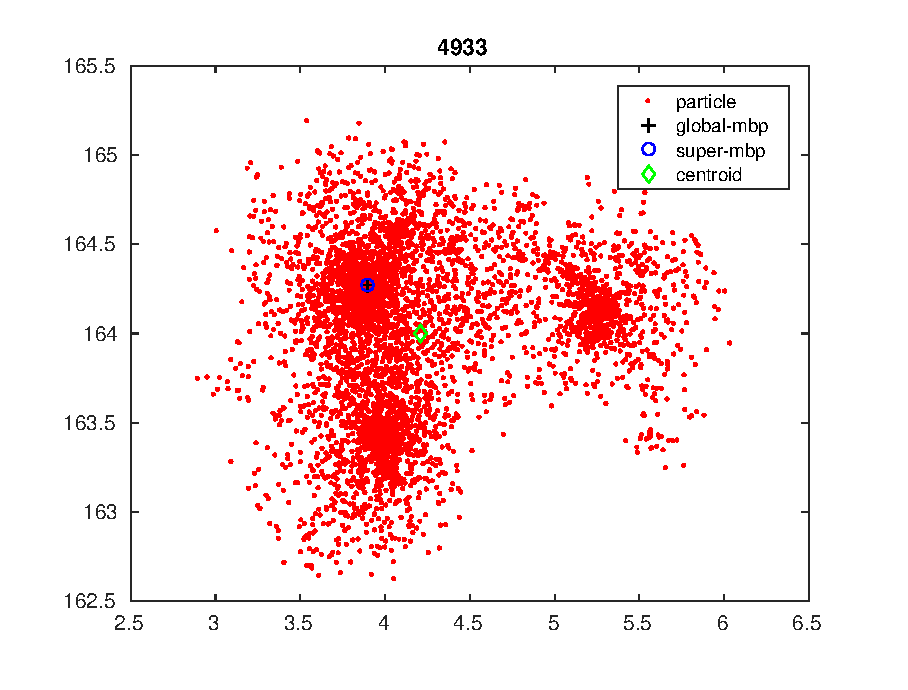
\includegraphics[scale=0.45]{2d_result}
\end{figure}
\end{columns}
}
\frame{
\frametitle{Results for 3D Halos}
\begin{columns}
\column{2.5in}
\begin{figure}[H]
\includegraphics[scale=0.5]{3d_timing}
\end{figure}
\column{2.5in}
\begin{figure}[H]
\centering
    \includegraphics[scale=0.5]{3d_error}
\end{figure}
\end{columns}
}
\section{Summary}
%  \begin{frame}
%    \frametitle{Outline}
%    \tableofcontents[currentsection]
%  \end{frame}

\frame{
\frametitle{Summary}
\begin{itemize}
  \item We propose a highly recursive algorithm to accelerate the process the halo MBP finding.
\vspace{12pt}
   \item Preliminary results show the potential of the proposed algorithm to reduce the complexity to $O(N_p \log N_p)$.
\vspace{12pt}
   \item There are still many components requiring rigorous analysis for optimal performance from both the mathematical and physical principles.
\vspace{12pt}
\end{itemize}
}
\frame{
\frametitle{Acknowledgement}
\begin{block}{}
This work was funded under the ECP codesign center ``Codar''. 
\end{block}
\vspace{12pt}

\begin{center}
\textcolor{red}{THANKS!}
\end{center}
}
\end{document}

